\begin{figure}[!tbp]
  \centering
  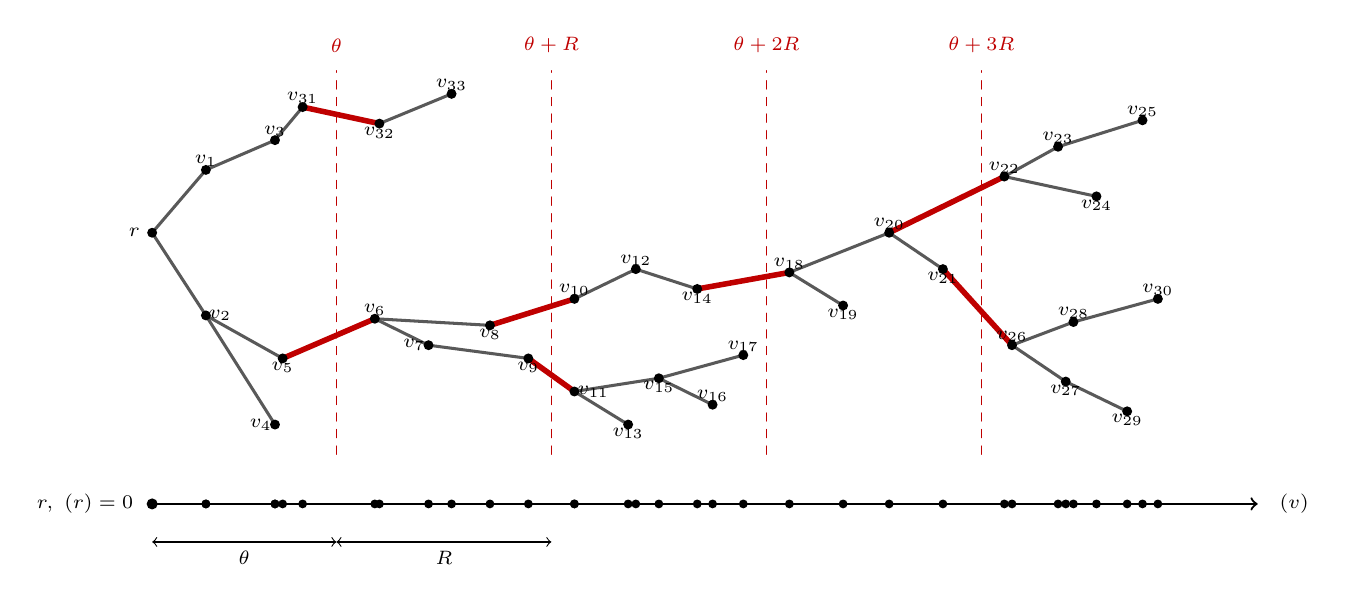
\begin{tikzpicture}[
    x=1.95cm,
    y=0.42cm,
    line cap=round,
    line join=round,
    treeedge/.style={draw=black!65,line width=1.1pt},
    cutedge/.style={draw=red!75!black,line width=2pt}
  ]
    % Horizontal position is D(v); vertical position gives a clean tree layout.
    \coordinate (rT) at (0,0);
    \coordinate (v1T) at (0.35,1.9);
    \coordinate (v2T) at (0.35,-2.5);
    \coordinate (v3T) at (0.8,2.8);
    \coordinate (v4T) at (0.8,-5.8);
    \coordinate (v5T) at (0.85,-3.8);
    \coordinate (v6T) at (1.45,-2.6);
    \coordinate (v7T) at (1.8,-3.4);
    \coordinate (v8T) at (2.2,-2.8);
    \coordinate (v9T) at (2.45,-3.8);
    \coordinate (v10T) at (2.75,-2.0);
    \coordinate (v11T) at (2.75,-4.8);
    \coordinate (v12T) at (3.15,-1.1);
    \coordinate (v13T) at (3.1,-5.8);
    \coordinate (v14T) at (3.55,-1.7);
    \coordinate (v15T) at (3.3,-4.4);
    \coordinate (v16T) at (3.65,-5.2);
    \coordinate (v17T) at (3.85,-3.7);
    \coordinate (v18T) at (4.15,-1.2);
    \coordinate (v19T) at (4.5,-2.2);
    \coordinate (v20T) at (4.8,0.0);
    \coordinate (v21T) at (5.15,-1.1);
    \coordinate (v22T) at (5.55,1.7);
    \coordinate (v23T) at (5.9,2.6);
    \coordinate (v24T) at (6.15,1.1);
    \coordinate (v25T) at (6.45,3.4);
    \coordinate (v26T) at (5.6,-3.4);
    \coordinate (v27T) at (5.95,-4.5);
    \coordinate (v28T) at (6.0,-2.7);
    \coordinate (v29T) at (6.35,-5.4);
    \coordinate (v30T) at (6.55,-2.0);
    \coordinate (v31T) at (0.98,3.8);
    \coordinate (v32T) at (1.48,3.3);
    \coordinate (v33T) at (1.95,4.2);

    % Four thresholds t_k = theta + k R, k=0,...,3.
    \foreach \x in {1.2,2.6,4.0,5.4} {
      \draw[red!75!black,dashed,thin] (\x,-6.7) -- (\x,4.9);
    }

    % The four thresholds cross 2, 2, 1, and 2 edges, respectively.
    \draw[treeedge] (rT) -- (v1T);
    \draw[treeedge] (rT) -- (v2T);
    \draw[treeedge] (v1T) -- (v3T);
    \draw[treeedge] (v3T) -- (v31T);
    \draw[cutedge] (v31T) -- (v32T);
    \draw[treeedge] (v32T) -- (v33T);
    \draw[treeedge] (v2T) -- (v4T);
    \draw[treeedge] (v2T) -- (v5T);
    \draw[cutedge] (v5T) -- (v6T);
    \draw[treeedge] (v6T) -- (v7T);
    \draw[treeedge] (v6T) -- (v8T);
    \draw[treeedge] (v7T) -- (v9T);
    \draw[cutedge] (v8T) -- (v10T);
    \draw[cutedge] (v9T) -- (v11T);
    \draw[treeedge] (v10T) -- (v12T);
    \draw[treeedge] (v12T) -- (v14T);
    \draw[treeedge] (v11T) -- (v13T);
    \draw[treeedge] (v11T) -- (v15T);
    \draw[treeedge] (v15T) -- (v16T);
    \draw[treeedge] (v15T) -- (v17T);
    \draw[cutedge] (v14T) -- (v18T);
    \draw[treeedge] (v18T) -- (v19T);
    \draw[treeedge] (v18T) -- (v20T);
    \draw[treeedge] (v20T) -- (v21T);
    \draw[cutedge] (v20T) -- (v22T);
    \draw[cutedge] (v21T) -- (v26T);
    \draw[treeedge] (v22T) -- (v23T);
    \draw[treeedge] (v22T) -- (v24T);
    \draw[treeedge] (v23T) -- (v25T);
    \draw[treeedge] (v26T) -- (v27T);
    \draw[treeedge] (v26T) -- (v28T);
    \draw[treeedge] (v27T) -- (v29T);
    \draw[treeedge] (v28T) -- (v30T);

    % Draw the tree vertices over the edges and threshold guides.
    \foreach \p in {rT,v1T,v2T,v3T,v4T,v5T,v6T,v7T,v8T,v9T,v10T,v11T,v12T,v13T,v14T,v15T,v16T,v17T,v18T,v19T,v20T,v21T,v22T,v23T,v24T,v25T,v26T,v27T,v28T,v29T,v30T,v31T,v32T,v33T} {
      \fill[black] (\p) circle (1.8pt);
    }
    \node[anchor=east,font=\scriptsize,inner sep=1pt] at (-0.06,0) {$r$};
    \node[anchor=south,font=\scriptsize,inner sep=1pt] at (0.35,1.9) {$v_1$};
    \node[anchor=west,font=\scriptsize,inner sep=1pt] at (0.35,-2.5) {$v_2$};
    \node[anchor=south,font=\scriptsize,inner sep=1pt] at (0.8,2.8) {$v_3$};
    \node[anchor=east,font=\scriptsize,inner sep=1pt] at (0.8,-5.8) {$v_4$};
    \node[anchor=north,font=\scriptsize,inner sep=1pt] at (0.85,-3.8) {$v_5$};
    \node[anchor=south,font=\scriptsize,inner sep=1pt] at (1.45,-2.6) {$v_6$};
    \node[anchor=east,font=\scriptsize,inner sep=1pt] at (1.8,-3.4) {$v_7$};
    \node[anchor=north,font=\scriptsize,inner sep=1pt] at (2.2,-2.8) {$v_8$};
    \node[anchor=north,font=\scriptsize,inner sep=1pt] at (2.45,-3.8) {$v_9$};
    \node[anchor=south,font=\scriptsize,inner sep=1pt] at (2.75,-2.0) {$v_{10}$};
    \node[anchor=west,font=\scriptsize,inner sep=1pt] at (2.75,-4.8) {$v_{11}$};
    \node[anchor=south,font=\scriptsize,inner sep=1pt] at (3.15,-1.1) {$v_{12}$};
    \node[anchor=north,font=\scriptsize,inner sep=1pt] at (3.1,-5.8) {$v_{13}$};
    \node[anchor=north,font=\scriptsize,inner sep=1pt] at (3.55,-1.7) {$v_{14}$};
    \node[anchor=north,font=\scriptsize,inner sep=1pt] at (3.3,-4.4) {$v_{15}$};
    \node[anchor=south,font=\scriptsize,inner sep=1pt] at (3.65,-5.2) {$v_{16}$};
    \node[anchor=south,font=\scriptsize,inner sep=1pt] at (3.85,-3.7) {$v_{17}$};
    \node[anchor=south,font=\scriptsize,inner sep=1pt] at (4.15,-1.2) {$v_{18}$};
    \node[anchor=north,font=\scriptsize,inner sep=1pt] at (4.5,-2.2) {$v_{19}$};
    \node[anchor=south,font=\scriptsize,inner sep=1pt] at (4.8,0.0) {$v_{20}$};
    \node[anchor=north,font=\scriptsize,inner sep=1pt] at (5.15,-1.1) {$v_{21}$};
    \node[anchor=south,font=\scriptsize,inner sep=1pt] at (5.55,1.7) {$v_{22}$};
    \node[anchor=south,font=\scriptsize,inner sep=1pt] at (5.9,2.6) {$v_{23}$};
    \node[anchor=north,font=\scriptsize,inner sep=1pt] at (6.15,1.1) {$v_{24}$};
    \node[anchor=south,font=\scriptsize,inner sep=1pt] at (6.45,3.4) {$v_{25}$};
    \node[anchor=south,font=\scriptsize,inner sep=1pt] at (5.6,-3.4) {$v_{26}$};
    \node[anchor=north,font=\scriptsize,inner sep=1pt] at (5.95,-4.5) {$v_{27}$};
    \node[anchor=south,font=\scriptsize,inner sep=1pt] at (6.0,-2.7) {$v_{28}$};
    \node[anchor=north,font=\scriptsize,inner sep=1pt] at (6.35,-5.4) {$v_{29}$};
    \node[anchor=south,font=\scriptsize,inner sep=1pt] at (6.55,-2.0) {$v_{30}$};
    \node[anchor=south,font=\scriptsize,inner sep=1pt] at (0.98,3.8) {$v_{31}$};
    \node[anchor=north,font=\scriptsize,inner sep=1pt] at (1.48,3.3) {$v_{32}$};
    \node[anchor=south,font=\scriptsize,inner sep=1pt] at (1.95,4.2) {$v_{33}$};

    % Distance-coordinate line with the matching vertices at the same x values.
    \draw[->,thick] (0,-8.2) -- (7.2,-8.2);
    \foreach \x in {0.35,0.35,0.8,0.8,0.85,0.98,1.45,1.48,1.8,1.95,2.2,2.45,2.75,2.75,3.1,3.15,3.3,3.55,3.65,3.85,4.15,4.5,4.8,5.15,5.55,5.6,5.9,5.95,6.0,6.15,6.35,6.45,6.55} {
      \fill[black] (\x,-8.2) circle (1.6pt);
    }
    \fill[black] (0,-8.2) circle (2pt);
      \node[anchor=east,font=\scriptsize] at (-0.06,-8.2) {$r,\ \dist(r)=0$};
      \node[anchor=west,font=\scriptsize] at (7.28,-8.2) {$\dist(v)$};

    \node[anchor=south,font=\scriptsize,text=red!75!black] at (1.2,5.15) {$\theta$};
    \node[anchor=south,font=\scriptsize,text=red!75!black] at (2.6,5.15) {$\theta+R$};
    \node[anchor=south,font=\scriptsize,text=red!75!black] at (4.0,5.15) {$\theta+2R$};
    \node[anchor=south,font=\scriptsize,text=red!75!black] at (5.4,5.15) {$\theta+3R$};

    % Show the first offset and one period between consecutive thresholds.
    \draw[<->,thin] (0,-9.35) -- (1.2,-9.35)
      node[midway,below=2pt,font=\scriptsize,fill=white,inner sep=1pt] {$\theta$};
    \draw[<->,thin] (1.2,-9.35) -- (2.6,-9.35)
      node[midway,below=2pt,font=\scriptsize,fill=white,inner sep=1pt] {$R$};
  \end{tikzpicture}
  \caption{The vertices in $V$ projected onto a line according to the $\dist_x(r,v)$ values and the placement of thresholds $\theta+kR$ for $k=0,\ldots,3$.}
  \label{fig:anchored-lp-threshold-line}
\end{figure}
